\section{Ergebnisse / Evaluation}
\begin{itemize}
	\item Skalierbarkeitsgraph
	\item Wie gut ist SIMD / OpenMP / MPI / Mischformen?
	\item Frontend Overhead messen
\end{itemize}


%%%%%%%
% http://www.caps.in.tum.de/himmuc/
% Datenerhebenung (+ auf himmuc!) -> Max
% Skalierungs bzgl anzahl an nodes
% Vergleich OpenMP und mehrere MPI pro Node -> Tobi
% Overhead durch Balancer -> Florian
% Overhead durch MPI / Websocket / DrawTiles (konstant)
% Vergleich SIMD / Rohcode -> Niels

% Nutzbarkeit/ HCI -> Max
% vergleich x86 -> Max
\subsection{Performanzerhöhung alternative Parallelisierungsmechanismen}

\subsubsection{Datenerhebung}
% Max
% Datenerhebung auf himmuc cluster
% Messen der Timings im backend (Wie kommen die Daten im frontend zu stande?)
% Auswahl der repräsentativen Punkte
% Grobes Intro zu der folgenden Evaluation

\subsubsection{Skalierung}

% Tobi
% MPI Skalierung
% Skalierungsgraph (Naiver Balancer, Maxcomputation time per Region vs Node count)
% 	3 Plots Regionen außen, Randregionen und Regionen in der Mitte
% 	Jeweils auf separater y-Achse Mpi time 
% Wie gut ist die MPI Kommunikation. Ab wann macht es keinen Sinn mehr, mehr Worker einzusetzen


% OpenMP & MPI skalierung
% Bar graph (1 MPI Prozess pro worker, 1 MPI Prozess & 4 OpenMP pro Worker, 4 MPI Prozesse pro worker)
% 	Worker & Iteration Anzahl fest, optimal wählen, Randregion


\subsubsection{SIMD (Implementierungen)}

% Niels:
% PLOTS: (mandelbrot 32, 64, simd 32,  64, 80 bit default)
% comp time vs iteration count plot
% speed up factor vs number of iterations
% (niedriger, höher ist besser)


% refactor:
% three bar graphs - average computation time for worst 25%, average 50% and best 50%
% one figure showing where SIMD achieves best increase in performance (see notebook)

SIMD unterstützt in den Präzisionen 32 und 64 bit Parallelisierung von einer Rechenoperationen auf
4 beziehungsweise 2 unterschiedlichen Werten. Der Effekt beläuft sich dabei, wie in \autoref{fig:SIMD-speedup} zu sehen,
auf eine durchschnittliche Beschleunigung um den Faktor 1,9 und 1,2.

\begin{figure}
	\centering
	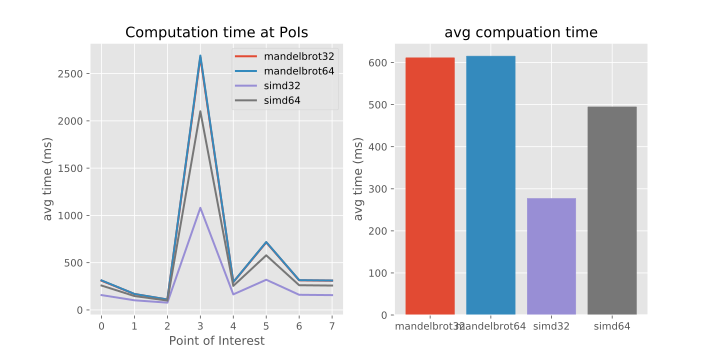
\includegraphics[width=0.9\linewidth]{img/Evaluation/impl_test}
	\caption{Vergleich der Performanzen der Implementierungen mit und ohne SIMD}
	\label{fig:SIMD-speedup}
\end{figure}

Dass die Performanzerhöhung nicht genau 4 oder 2 ist, lässt sich mit dem Erhöhten Aufwand der Verwendung
der SIMD Instruktionen erklären.
Da hierzu die Werte aus den normalen Registern in spezielle SIMD-Register und zurück
kopiert werden müssen, entsteht eine gewisse Verzögerung durch zusätzliche Transportoperationen.
Die tatsächliche Rechenzeit für eine Vektorisierung von \(n\) Punkten sollte also \autoref{equ:simd-time} entsprechen.

\begin{equation}\label{equ:simd-time}
	t_{SIMD} \approx \frac{t_{normal}}{n}+ const
\end{equation}

Je größer die benötigte Zahl an Operationen, desto weniger fällt dieser konstante Zusatzaufwand ins Gewicht.
Dies kann zum Beispiel in \autoref{fig:SIMD-speedup-vs-comptime} beobachtet werden.

Zudem werden für eine Menge an Punkten stets die Zahl an Iterationen durchgeführt,
die das Maximum aller Iterationszahlen der Punkte ist.
Bei Iterationszahlen \(i_k\) des Punktvektors \(p\) ist daher
anstatt einer Rechenzeit von \(\sum_{k \in p} \frac{i_k }{ | p | }\) eine Rechenzeit von
\(\sum_{k \in p} \frac{max(i_k)_{k \in p }}{|p|} = max(i_k)_{k \in p }\) pro Punktvektor zu erwarten.
Damit wird die Beschleunigung durch SIMD kleiner, je inhomogener die Iterationszahlen sind.
Dass die Iterationszahlen im Allgemeinen am Rand der Mandelbrotmenge inhomogener sind,
wo auch die Gesamtrechenzeit geringer ist, sollte bei der Betrachtung von \autoref{fig:SIMD-speedup-vs-comptime} berücksichtigt werden.

\begin{figure}
	\centering
	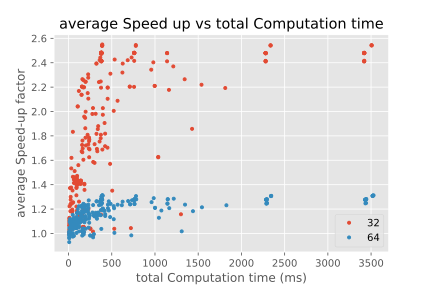
\includegraphics[width=0.9\linewidth]{img/Evaluation/speedupvscomptime}
	\caption{Beschleunigungsfaktor durch SIMD in Abhängigkeit von der durchschnittlichen Rechenzeit}
	\label{fig:SIMD-speedup-vs-comptime}
\end{figure}

\paragraph{Notiz, entdeckt durch das In-Betracht-Ziehen der Leerregionen}

Probleme bei der Verwendung des Rekursiven Lastbalanierers:
Da es stets im Diskreten eine Minimalgröße für die aufgeteilten Regionen gibt,
kann es sein, dass eine Region für die eine hohe Last vorhergesagt wird viele Worker reserviert -
diese jedoch nicht vollständig ausreizen kann, da die Maximalaufteilung schon erreicht wurde.
Durch die dadurch entstehenden Leerregionen von nicht verwendbaren Workern
kann eine suboptimale Aufteilung enstehen, schlechter noch als die des naiven rekursiven Balancierers.

Dies kann abgeschwächt werden, indem eine Region stets nur soviel Workerressourcen erhält,
wie sie maximal auslasten könnte (Fläche/Fläche minimaler Aufteilung)


\subsubsection{Balancer}

% Florian
% Wir haben zwei Klassen (naive, prediction) und wählen davon jeweils den besten 
% (naive Recursive, prediction Recursive)

% Erst naiver Balancer, dann prediction dafür jeweils:
% 	Plot der distribution function (Median, Max)
% 	Maximale Rechenzeit & Wie gut sind die Werte um den Median verteilt
% 	3 Plots mit Regionen außerhalb, im Rand und innerhalb der Mandelbrotmenge

% Genauigkeit der Vorhersage vs maximale Rechenzeit für Randregionen 
	% Plot: y: max comp time, balancer time  x: prediction Accuracy (Randregion)
% 	Diese "optimale" Genauigkeit wird aber bereits in allen vorherigen Evaluierungen des  prediction Balancers verwendet

% Florian: Predictionaccuracy im Backend dynamisch auswählbar machen

\subsubsection{Didaktik}
% Max
% Konstanter Overhead wurde getestet,
% auf himmuc leider nicht so gut erkennbar, da Netzwerk overhead zu groß ist.
% Lokal nicht so ein Problem. Somit würde das Programm auf superMUC seinen Zweck erfüllen.

\subsubsection{Zusammenfassung}
% Speedup
% Kombinationen von Unterschiedlichen Verbesserungen. als Plot.
% (Eine Klasse von Regionen)